\chapter{NOOSFERO}

O Noosfero é uma plataforma \textit{open source} para a construção de redes sociais
e colaborativas. Desenvolvido em Ruby on Rails e licenciado sob AGPL versão 3, o
projeto conta com desenvolvimento ativo.

Além dos mecanismos de interação social, o Noosfero também conta com um sistema de
gerenciamento de conteúdo, o que possibilita a criação de \textit{blogs} e o
compartilhamento de arquivos. A plataforma também pode ser estendida por
\textit{plugins} desenvolvidos pela comunidade, e conta com o conceito de ambientes,
que permitem a criação de diversas redes isoladas funcionando sobre uma mesma
instância da aplicação.

\begin{figure}[h]
	\centering
		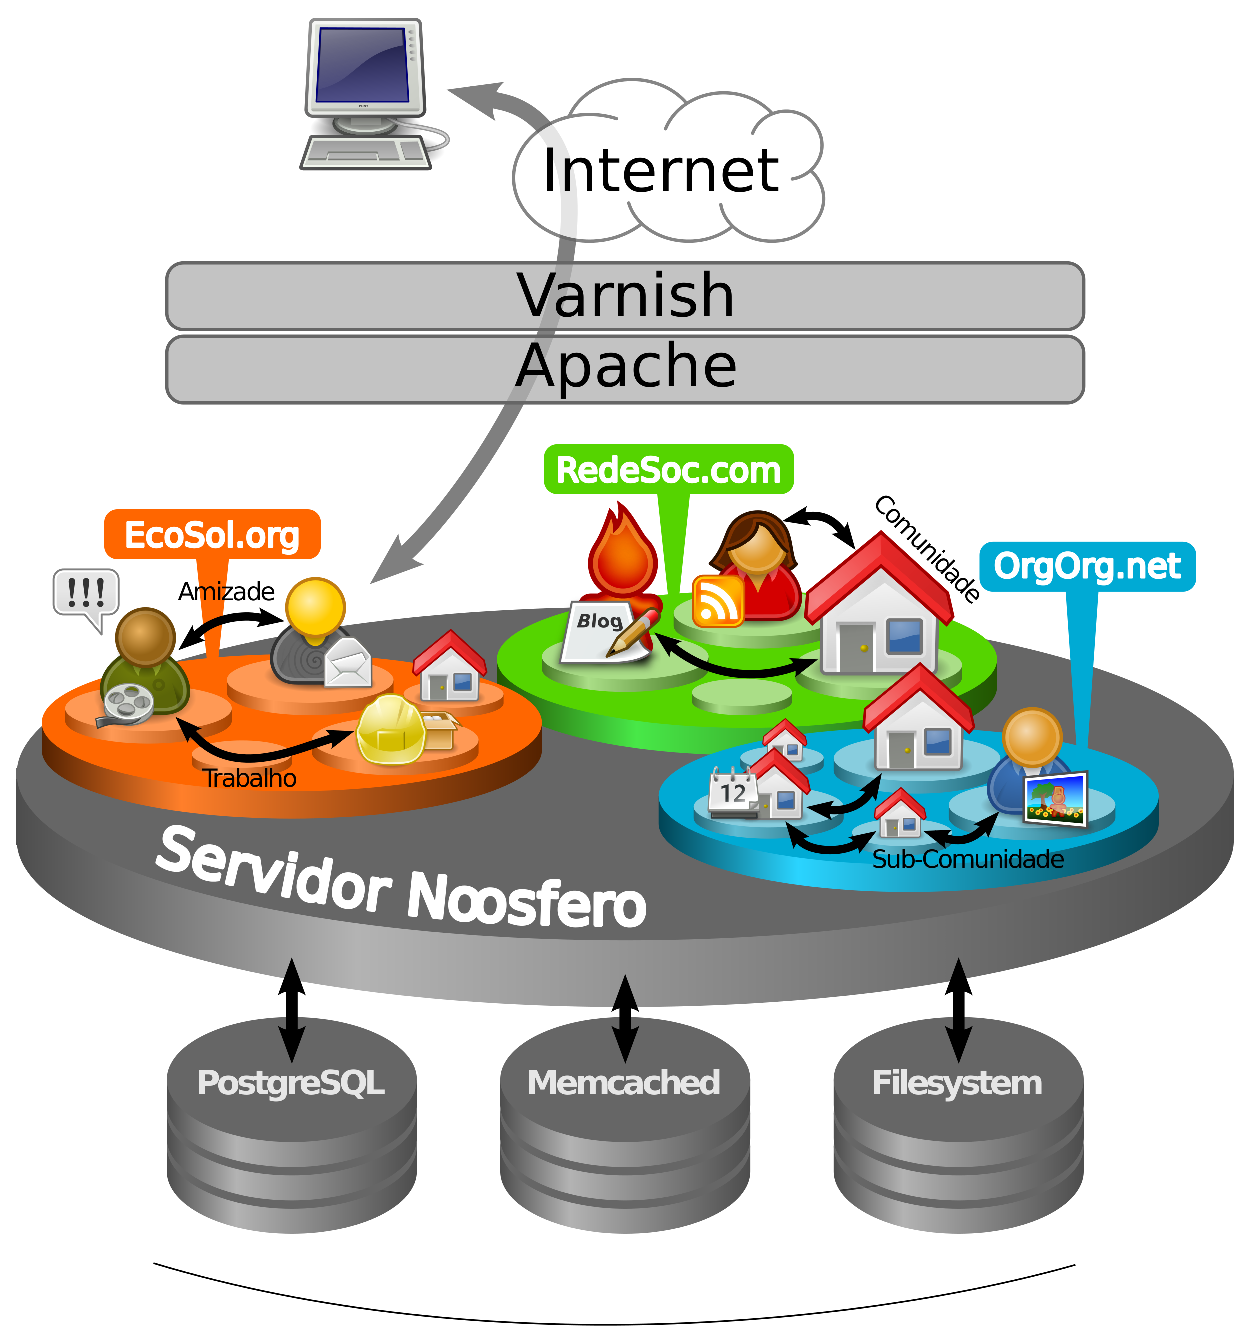
\includegraphics[keepaspectratio=true,scale=0.4]{figuras/noosfero_estrutura.eps}
	\caption{Arquitetura do Noosfero}
	\label{fig:noosferoEstrutura}
\end{figure}
% adicionar fonte

As informações e publicações de pessoas e organizações podem ser públicas ou
privadas. Já os relacionamentos entre estas entidades podem ser tanto simétricos
como assimétricos.

Enquanto um relacionamento simétrico depende da concordância de ambas as partes para
o compartilhamento das informações privadas (como por exemplo amizades ou
filiações), um relacionamento assimétrico depende apenas do interesse de uma das
entidades em acompanhar as informações públicas de algum perfil (como no caso da
funcionalidade de seguidores).



\section{SUPORTE À FEDERAÇÃO}

As definições da federação no Noosfero surgiram no contexto de desenvolvimento do
projeto do Portal do Software Público, como resultado de uma consultoria executada
pela Cooperativa de Tecnologias Livres \cite{colivre2016}. O produto foi um
relatório que define os objetivos e requisitos da implementação de federação na
plataforma Noosfero.

A proposta é que seja possível realizar a integração não só com outras instâncias do
Noosfero, como também com outras redes sociais. Desta forma, é necessário adotar
especificações que tenham o mínimo de aderência na comunidade, ao menos em outros
projetos que investem na implementação da federação entre redes sociais. Os
protocolos Diaspora e OStatus foram escolhidos observando projetos como o Hubzilla,
Friendica, e o próprio Diaspora.

É interessante que mesmo a integração entre redes Noosfero respeite os padrões
adotados pelos protocolos de referência, evitando a criação de outro padrão que não
reconhecido pelo restante dos projetos. No entanto, implementar a federação
respeitando os padrões existentes pode exigir uma refatoração da arquitetura ou das
funcionalidades da plataforma. Por exemplo, nenhum dos protocolos de referência
respeita o conceito de relacionamentos simétricos, padrão no Noosfero até então.


\subsection{Federação entre redes Noosfero}

As primeiras contribuições com a federação no Noosfero foram na integração de
instâncias diferentes da plataforma. As atividades foram definidas de acordo com
um \textit{roadmap} que dividiu a implementação em quatro fases, que cobrem desde
a reestruturação da arquitetura da aplicação, até a construção dos mecanismos
necessários para a autenticação e relação entre as redes.

Foi definido que um usuário de uma rede Noosfero pode acessar qualquer outra
instância com as credenciais de sua rede de origem. Um usuário federado deve ser
capaz de visualizar conteúdos públicos, comentar publicações, seguir usuários, e
deixar mensagens em murais. As notificações destas interações devem ser entregues
tanto aos usuários na rede local, quanto ao usuário na rede de origem.

O protocolo construído entre redes Noosfero é baseado nas especificações do
WebFinger e OAuth para a descoberta de identidade e autorização de perfis,
respectivamente. Em relação à comunicação entre as redes, o protocolo Diaspora foi
definido como referência. 

\subsubsection{Fase 1: preparação}

Até a versão 1.5 do Noosfero, todos os relacionamentos entre as entidades da rede
eram baseados no conceito de relacionamento simétrico. No entanto, as demais redes
federadas, e a maioria dos padrões mais implementados, trabalham apenas com o
conceito de relacionamentos assimétricos, o que incentivou o desenvolvimento da
funcionalidade de seguidores no Noosfero.

Na fase de preparação foram introduzidos os relacionamentos assimétricos através
desta funcionalidade. Os seguidores são notificados a respeito de atividades
públicas de perfis seguidos. No Noosfero, cada perfil pode permitir ou não que
usuários o sigam. Usuários por sua vez organizam seus seguidores em círculos,
categorizando suas relações.

\subsubsection{Fase 2: intercomunicações}

Durante a fase de intercomunicações foi construída a infraestrutura básica para a
integração entre redes Noosfero. Ambientes e usuários externos foram introduzidos à
arquitetura do Noosfero, que passa a considerar a ação de usuários que não possuem
perfis locais sobre a aplicação.

% Explicar o modelo do Noosfero antes desta seção?
O conceito de usuário externo, introduzido nesta fase, é importante para toda a
implementação da federação do Noosfero. Um usuário local do Noosfero é definido por
basicamente dois objetos de negócio --- um usuário, que armazena as credenciais de
acesso, e um perfil, que armazena suas demais informações na aplicação, sendo o que
de fato se relaciona com o restante do domínio.

Já o usuário externo não possui credenciais de acesso na instância visitada, apenas
um objeto que representa o seu perfil externo, e que do ponto de vista da
implementação deve ser capaz de reproduzir o comportamento de um perfil comum. A
implementação alcançada faz uso de métodos \textit{stub} e relações polimórficas.

Nesta fase também foi implementada a especificação do WebFinger, que já está sendo
utilizada para a descoberta de usuários na autenticação entre redes Noosfero.

% TODO: adicionar nota de rodapé com directory.noosfero.org
Inicialmente, apenas as redes listadas no diretório central do Noosfero podem ser
habilitadas no painel de administração da federação. A descentralização desta lista
ou a automatização do processo de descoberta não fizeram parte do planejamento
inicial.

\subsubsection{Fase 3: integração externa}

A fase de integração externa teve como objetivo aproveitar a infraestrutura de
usuários externos para autenticar usuários de outros serviços sem a necessidade de
perfis locais. Com isto, usuários de sistemas que suportem OAuth podem acessar o
Noosfero, consumir conteúdo, e executar um conjunto limitado de ações.

Durante esta etapa, o \textit{plugin} que torna o Noosfero em um cliente OAuth foi
evoluído para permitir que usuários possam tanto criar um perfil local a partir das
informações da rede de origem, como também apenas acessar o Noosfero com um perfil
temporário. Por enquanto, os únicos fornecedores OAuth suportados são o Google,
Facebook, Twitter, GitHub, e o próprio Noosfero. No entanto, novos fornecedores
podem ser facilmente adicionados.

\subsubsection{Fase 4: inter-relações}

A última fase de desenvolvimento da federação de redes Noosfero foi implementar o
relacionamento entre usuários de instâncias diferentes. De modo geral, esta fase
consistiu em permitir que usuários externos sejam capazes de seguir perfis, comentar
conteúdos, e publicar em murais de outros usuários.

De forma a permitir relações entre usuários federados foi necessário refatorar a
funcionalidade de seguidores, adicionando o suporte a perfis externos. Neste ponto,
usuários federados podem tanto seguir usuários locais, quanto serem seguidos por
eles. A necessidade de simetria se dá pela contabilização e exibição dos perfis
seguidores e seguidos.

% TODO: explicar o mecanismo de troca de mensagens
Também foi necessário implementar uma infraestrutura de troca de mensagens entre
instâncias do Noosfero, possibilitando o envio das notificações necessárias para o
estabelecimento das interações.


\subsection{Federação com outras redes sociais}

A implementação da federação com redes não Noosfero devem usar a infraestrutura
desenvolvida para a integração entre redes Noosfero, principalmente os mecanismos
de usuários externos e troca de mensagens.

Já que não existe um padrão para a federação de redes sociais, inicialmente é
necessário oferecer suporte a aplicações individuais. Dedicou-se atenção especial
aos projetos que contam com iniciativas de federação significativas, precisamente
os projetos Diaspora, Hubzilla, Friendica, e GNU Social. Estes projetos foram
escolhidos pela atividade e maturidade da discussão das comunidades e pela aderência
de outras aplicações, o que seria um indicador da susceptibilidade ao surgimento de
possíveis padrões.

Com exceção do GNU Social, os projetos que serão inicialmente suportados atendem às
especificações do protocolo Diaspora. O suporte às redes baseadas no OStatus poderia
ser oferecido implementando uma parte dos protocolos desta suíte, como o Salmon, o
Activity Streams, e o PubHubSub.

Para que a federação seja bem sucedida, é essencial garantir que a integração seja
bidirecional. Além de permitir que usuários acessem e interajam com uma rede
Noosfero com o perfil de outra rede social, um usuário Noosfero também devem
conseguir fazer o mesmo em qualquer uma destas redes. Além da autorização, a
federação depende da descentralização dos conteúdos, o que exige que as interações
possam acontecer em qualquer uma das redes e que o estado seja sempre o mesmo em
cada uma delas.

De modo geral, as mesmas funcionalidades implementadas na federação de redes
Noosfero deve ser suportada, desde que toda interação exerça impacto tanto na rede
de origem quanto na rede federada, sejam estas instâncias Noosfero ou não.

As atividades necessárias para a implementação desta etapa de federação podem ser
organizadas com base nos marcos a seguir.

\begin{enumerate}
  \item{Possibilitar um usuário possa acessar outras redes com as credenciais de sua
        rede de origem, sem a necessidade de um novo cadastro. Inicialmente, deve-se
        desenvolver um \textit{plugin} para autorização com OpenID, visto que é o
        único padrão implementado pelo Diaspora;}

  \item{Permitir que usuários de outras redes possam ser encontrados através da
        busca do Noosfero, o que é o primeiro passo para as inter-relações. A busca
        deve respeitar o padrão de descoberta do Diaspora, baseado no WebFinger;}

  \item{Implementar relações assimétricas entre os usuários do Noosfero e de redes
        que respondam ao protocolo Diaspora. O protocolo deve ser usado para que as
        duas redes estejam cientes da relação;}

  \item{Permitir que o Noosfero receba as publicações enviadas por redes que
        implementem o protocolo Diaspora. O Noosfero também deve ser capaz de enviar
        novos conteúdos a estas redes;}

  % Retração de relacionamentos?
  % Exclusão de conteúdos?
  % Menções? Compartilhamentos? Mensagens diretas?

  \item{Implementar o envio de mensagens através dos padrões Salmon e PubHubSub,
        garantindo a federação dos conteúdos com redes que respondam ao padrão
        OStatus;}
\end{enumerate}

% TODO: (no caso do Diaspora: o que inclui tais e tais funcionalidades...)
No desenvolvimento deste trabalho será priorizada a implementação da federação
através do protocolo Diaspora. Indica-se a expansão da federação por meio do OStatus
como um trabalho futuro.

\subsubsection{Implementação do Protocolo Diaspora}

O protocolo Diaspora está implementado no formato de uma \textit{gem}, que pode ser
facilmente incorporado como dependência em projetos desenvolvidos em linguagem Ruby,
como o Noosfero. A \textit{gem} é mantida pela mesma comunidade responsável pelo
projeto original, e sempre acompanha a última especificação adotada.

Segundo os mantenedores, o protocolo Diaspora ainda não está estável, e alterações
capazes de introduzir incompatibilidades podem ser introduzidas na \textit{gem}. A
implementação inicial no Noosfero deve ser executada sobre a última versão estável
disponível no momento de sua adição ao projeto.

% TODO: adicionar nota para o hcard
O primeiro elemento necessário para a implementação da interoperabilidade é um
mecanismo de descoberta de informações entre servidores, no caso do Diaspora o
WebFinger. A implementação base já está disponível no Noosfero, sendo necessário
testar a integração com outro sistema que implemente o protocolo. Neste ponto a
especificação do Diaspora também exige que a resposta WebFinger inclua um
\textit{hcard}, que por sua vez contém informações pessoais de cada usuário, e
também deve ser implementado no Noosfero.

O segundo elemento é a comunicação entre os servidores, realizada através da troca
de mensagens contendo entidades, que representam as interações entre os usuários e
conteúdos. É importante que o Noosfero reconheça as entidades listadas a seguir.

\begin{itemize}
  \item{Perfil de usuário e atualizações}
  \item{Publicações e respostas}
  \item{Participação (inscrição em publicações)}
  \item{Contato entre usuários (seguir ou deixar de seguir)}
  \item{Retração das entidades listadas}
\end{itemize}

As mensagens são transferidas entre os servidores por meio do protocolo Salmon. A
\textit{gem diaspora\char`_federation} provê as funcionalidades de criptografia e
serialização necessárias para a comunicação sobre este padrão, e será adicionada
como dependência do Noosfero para auxiliar a implementação do protocolo Diaspora.

